\documentclass[11pt, a4paper]{article}

% Fonts and Encoding
\usepackage[utf8]{inputenc}
\usepackage[T1]{fontenc}
\usepackage{lmodern}

% Math and Symbols
\usepackage{amsmath, amssymb, amsthm, amsfonts, mathrsfs, mathtools}

% Layout and Geometry
\usepackage{geometry}
\geometry{a4paper, margin=1in}

% Formatting and Graphics
\usepackage{graphicx, xcolor, enumitem, booktabs, array, tabularx}

% TikZ for Illustrations
\usepackage{tikz}
\usetikzlibrary{arrows.meta, positioning, shapes.geometric, calc, backgrounds, matrix}

% Clickable Links and TOC
\usepackage{hyperref}
\hypersetup{
    colorlinks=true,
    linkcolor=blue,
    filecolor=magenta,      
    urlcolor=cyan,
    pdftitle={Advanced Mathematics Topic},
}

% Theorem Environments
\newtheorem{theorem}{Theorem}[section]
\newtheorem{lemma}[theorem]{Lemma}
\newtheorem{proposition}[theorem]{Proposition}
\newtheorem{corollary}[theorem]{Corollary}
\theoremstyle{definition}
\newtheorem{definition}{Definition}[section]
\newtheorem{axiom}{Axiom}[section]
\newtheorem{example}{Example}[section]
\theoremstyle{remark}
\newtheorem{remark}{Remark}[section]

% Custom Commands (Enforced standard notation)
\newcommand{\R}{\mathbb{R}}
\newcommand{\N}{\mathbb{N}}
\newcommand{\Z}{\mathbb{Z}}
\newcommand{\Q}{\mathbb{Q}}
\newcommand{\E}{\mathbb{E}}
\newcommand{\Prob}{\mathbb{P}}
\newcommand{\F}{\mathcal{F}}

\title{\textbf{Advanced Abstract Mathematics: Injective, Surjective, and Bijective Functions}}
\author{Tashfeen Omran}
\date{\today}

\begin{document}

\maketitle
\tableofcontents
\newpage

\section{Comprehensive Introduction, Context, and Prerequisites}

\subsection{Core Concepts and Axioms}
At the heart of modern abstract mathematics lies the concept of a \textit{function} (or mapping). A function $f$ from a set $A$ (the domain) to a set $B$ (the codomain), denoted as $f: A \to B$, is a fundamental set-theoretic relation that assigns to every element $x \in A$ exactly one element $y \in B$. We write this assignment as $f(x) = y$. 

While the definition of a function guarantees that every input has a unique output, it imposes no restrictions on how the outputs are distributed in the codomain. To classify the structural behavior of functions, we introduce three foundational properties:
\begin{itemize}
    \item \textbf{Injective (One-to-One):} A function $f: A \to B$ is injective if it never maps distinct elements of its domain to the same element of its codomain. Formally, $\forall a, b \in A$, if $f(a) = f(b)$, then $a = b$. Equivalently, by contrapositive, if $a \neq b$, then $f(a) \neq f(b)$.
    \item \textbf{Surjective (Onto):} A function $f: A \to B$ is surjective if its image covers the entire codomain. Formally, $\forall y \in B$, $\exists x \in A$ such that $f(x) = y$. In set-theoretic terms, the image of the domain $f(A)$ is exactly equal to $B$.
    \item \textbf{Bijective (One-to-One Correspondence):} A function is bijective if it is both injective and surjective. A bijection establishes a perfect pairing between the elements of $A$ and $B$, implying that the sets have the same cardinality (size).
\end{itemize}

\subsection{Intuition and Set-Theoretic Foundations}
To visualize these concepts, imagine the domain $A$ as a set of arrows and the codomain $B$ as a set of targets. A valid function requires every arrow to be shot exactly once. 
\begin{itemize}
    \item \textbf{Injectivity} means no two arrows hit the same target. Every target is hit at most once.
    \item \textbf{Surjectivity} means every target is hit by at least one arrow. No target is left empty.
    \item \textbf{Bijectivity} means every target is hit exactly once. This is only possible if the number of arrows perfectly matches the number of targets.
\end{itemize}
In advanced mathematics, bijections are the bedrock of \textit{isomorphisms}—mappings that preserve structural properties between abstract spaces, allowing mathematicians to treat seemingly different mathematical objects as fundamentally identical.

\subsection{Historical Context and Motivation}
The formalization of functions and their properties emerged during the late 19th century, driven by Georg Cantor's development of Set Theory. Prior to Cantor, functions were largely viewed as continuous algebraic formulas (e.g., $f(x) = x^2$). Cantor expanded this to arbitrary mappings between infinite sets. He used bijections to rigorously define the "size" (cardinality) of infinite sets, leading to the groundbreaking discovery that there are different sizes of infinity (e.g., the real numbers are uncountably infinite, whereas the integers are countably infinite). This sparked a foundational crisis in mathematics, ultimately resolved by the rigorous axiomatic frameworks of Zermelo-Fraenkel set theory.

\subsection{Key Theorems and Lemmas}
\begin{theorem}[Pigeonhole Principle for Finite Sets]
Let $A$ and $B$ be finite sets. 
\begin{enumerate}
    \item If $|A| > |B|$, then no function $f: A \to B$ can be injective.
    \item If $|A| < |B|$, then no function $f: A \to B$ can be surjective.
    \item If $|A| = |B|$, then a function $f: A \to B$ is injective if and only if it is surjective.
\end{enumerate}
\end{theorem}

\begin{theorem}[Composition of Functions]
Let $f: A \to B$ and $g: B \to C$ be functions.
\begin{enumerate}
    \item If $f$ and $g$ are injective, then $g \circ f$ is injective.
    \item If $f$ and $g$ are surjective, then $g \circ f$ is surjective.
\end{enumerate}
\end{theorem}

\subsection{Prerequisites}
To fully grasp this chapter, the reader must be proficient in:
\begin{itemize}
    \item \textbf{Basic Set Theory:} Understanding subsets, unions, intersections, and Cartesian products.
    \item \textbf{First-Order Logic:} Mastery of universal ($\forall$) and existential ($\exists$) quantifiers, implications, and contrapositives.
    \item \textbf{Proof Techniques:} Direct proof, proof by contradiction, and providing counterexamples.
    \item \textbf{Modular Arithmetic:} Basic understanding of divisibility and congruences.
\end{itemize}

\newpage
\section{Detailed Homework Solutions}

\subsection{Problem 10.18}
\textbf{Problem:} Let $A = \{w, x, y, z\}$ and $B = \{r, s, t\}$. Give an example of a function $f : A \to B$ that is neither one-to-one nor onto. Explain why $f$ fails to have these properties.

\textbf{Solution:}
We define the function $f: A \to B$ explicitly by mapping every element in the domain $A$ to a single element in the codomain $B$. Let:
\[ f = \{(w, r), (x, r), (y, r), (z, r)\} \]
\begin{proof}[Proof of non-injectivity]
A function is one-to-one if $f(a) = f(b) \implies a = b$. In our defined function, observe that $f(w) = r$ and $f(x) = r$. Thus, $f(w) = f(x)$, but $w \neq x$. Therefore, $f$ is not one-to-one.
\end{proof}
\begin{proof}[Proof of non-surjectivity]
A function is onto if for every $y \in B$, there exists an $a \in A$ such that $f(a) = y$. Consider the element $s \in B$. By our definition of $f$, the image of $A$ is $f(A) = \{r\}$. Since $s \notin \{r\}$, there is no element $a \in A$ such that $f(a) = s$. Therefore, $f$ is not onto.
\end{proof}

\subsection{Problem 10.19}
\textbf{Problem:} Give an example of two finite sets $A$ and $B$ and two functions $f : A \to B$ and $g : B \to A$ such that $f$ is one-to-one but not onto and $g$ is onto but not one-to-one.

\textbf{Solution:}
Let $A = \{1\}$ and $B = \{1, 2\}$. 
We define $f: A \to B$ as $f(1) = 1$.
We define $g: B \to A$ as $g(1) = 1$ and $g(2) = 1$.

\begin{proof}[Analysis of $f$]
To check if $f$ is one-to-one, we assume $f(a) = f(b)$. Since the only element in $A$ is $1$, $a$ and $b$ must both be $1$, so $a = b$. Thus, $f$ is one-to-one. To check if $f$ is onto, we look at the codomain $B$. The element $2 \in B$ has no pre-image in $A$ because $f(1) = 1 \neq 2$. Thus, $f$ is not onto.
\end{proof}
\begin{proof}[Analysis of $g$]
To check if $g$ is onto, we take an arbitrary element from the codomain $A$. The only element is $1$. We see that $g(1) = 1$, so a pre-image exists. Thus, $g$ is onto. To check if $g$ is one-to-one, we observe that $g(1) = 1$ and $g(2) = 1$. Since $g(1) = g(2)$ but $1 \neq 2$, $g$ is not one-to-one.
\end{proof}

\subsection{Problem 10.20}
\textbf{Problem:} A function $f : \Z \to \Z$ is defined by $f(n) = 2n + 1$. Determine whether $f$ is (a) injective, (b) surjective.

\textbf{Solution:}
\begin{proof}[Part (a): Injectivity]
Let $a, b \in \Z$ and assume $f(a) = f(b)$. We proceed via direct algebraic manipulation:
\begin{align*}
2a + 1 &= 2b + 1 \\
2a &= 2b \\
a &= b
\end{align*}
Since $f(a) = f(b) \implies a = b$, the function $f$ is injective.
\end{proof}
\begin{proof}[Part (b): Surjectivity]
We must determine if for every $y \in \Z$, there exists an $n \in \Z$ such that $f(n) = y$. Let $y = 2 \in \Z$. We set up the equation:
\begin{align*}
2n + 1 &= 2 \\
2n &= 1 \\
n &= \frac{1}{2}
\end{align*}
Since $n = 1/2 \notin \Z$, there is no integer $n$ that maps to $2$. Therefore, $f$ is not surjective.
\end{proof}

\subsection{Problem 10.21}
\textbf{Problem:} A function $f : \Z \to \Z$ is defined by $f(n) = n - 3$. Determine whether $f$ is (a) injective, (b) surjective.

\textbf{Solution:}
\begin{proof}[Part (a): Injectivity]
Let $a, b \in \Z$ and assume $f(a) = f(b)$. Then:
\begin{align*}
a - 3 &= b - 3 \\
a &= b
\end{align*}
Thus, $f$ is injective.
\end{proof}
\begin{proof}[Part (b): Surjectivity]
Let $y \in \Z$ be an arbitrary integer in the codomain. We need to find an $n \in \Z$ such that $f(n) = y$. We set $n - 3 = y$, which yields $n = y + 3$. Since the integers are closed under addition, and both $y$ and $3$ are integers, $n = y + 3 \in \Z$. Evaluating the function at this $n$ gives:
\[ f(y + 3) = (y + 3) - 3 = y \]
Since we found a valid integer pre-image for an arbitrary $y$, $f$ is surjective.
\end{proof}

\subsection{Problem 10.22}
\textbf{Problem:} A function $f : \Z \to \Z$ is defined by $f(n) = 5n + 2$. Determine whether $f$ is (a) injective, (b) surjective.

\textbf{Solution:}
\begin{proof}[Part (a): Injectivity]
Let $a, b \in \Z$ and assume $f(a) = f(b)$. Then:
\begin{align*}
5a + 2 &= 5b + 2 \\
5a &= 5b \\
a &= b
\end{align*}
Thus, $f$ is injective.
\end{proof}
\begin{proof}[Part (b): Surjectivity]
Let $y = 0 \in \Z$. We search for an $n \in \Z$ such that $f(n) = 0$.
\begin{align*}
5n + 2 &= 0 \\
5n &= -2 \\
n &= -\frac{2}{5}
\end{align*}
Since $-2/5 \notin \Z$, there is no integer $n$ that maps to $0$. Thus, $f$ is not surjective.
\end{proof}

\subsection{Problem 10.23}
\textbf{Problem:} Prove or disprove: For every nonempty set $A$, there exists an injective function $f : A \to \mathcal{P}(A)$.

\textbf{Solution:}
The statement is \textbf{True}. We will prove this by explicitly constructing an injective function.
\begin{proof}
Let $A$ be an arbitrary nonempty set. We define the function $f: A \to \mathcal{P}(A)$ by $f(x) = \{x\}$ for all $x \in A$. 
First, we verify that $f$ is well-defined. Since $x \in A$, the singleton set $\{x\}$ is a subset of $A$. By definition of the power set, $\{x\} \in \mathcal{P}(A)$. Thus, the codomain is correct.
Next, we prove injectivity. Let $a, b \in A$ and assume $f(a) = f(b)$. By our definition of $f$, this means:
\[ \{a\} = \{b\} \]
By the Axiom of Extensionality in set theory, two sets are equal if and only if they contain exactly the same elements. The only element in the set $\{a\}$ is $a$. Since the sets are equal, $a$ must also be an element of $\{b\}$. The only element in $\{b\}$ is $b$. Therefore, we must have $a = b$. 
Since $f(a) = f(b) \implies a = b$, the function $f$ is injective. $\blacksquare$
\end{proof}

\subsection{Problem 10.24}
\textbf{Problem:} Determine whether the function $f : \R \to \R$ defined by $f(x) = x^2 + 4x + 9$ is (a) one-to-one, (b) onto.

\textbf{Solution:}
We begin by completing the square to better understand the function's behavior:
\[ f(x) = (x^2 + 4x + 4) + 5 = (x + 2)^2 + 5 \]
\begin{proof}[Part (a): One-to-one]
We look for a counterexample. Let $a = 0$ and $b = -4$. 
\begin{align*}
f(0) &= (0 + 2)^2 + 5 = 4 + 5 = 9 \\
f(-4) &= (-4 + 2)^2 + 5 = (-2)^2 + 5 = 4 + 5 = 9
\end{align*}
Since $f(0) = f(-4)$ but $0 \neq -4$, the function is not one-to-one.
\end{proof}
\begin{proof}[Part (b): Onto]
We look for a counterexample in the codomain. Let $y = 0 \in \R$. We attempt to solve $f(x) = 0$:
\begin{align*}
(x + 2)^2 + 5 &= 0 \\
(x + 2)^2 &= -5
\end{align*}
In the real numbers, the square of any quantity is non-negative (i.e., $(x+2)^2 \ge 0$). Therefore, there is no real number $x$ that satisfies this equation. Since $0$ has no pre-image, $f$ is not onto.
\end{proof}

\subsection{Problem 10.25}
\textbf{Problem:} Is there a function $f : \R \to \R$ that is onto but not one-to-one? Explain your answer.

\textbf{Solution:}
Yes, such a function exists. 
\begin{proof}
Consider the cubic polynomial function $f(x) = x^3 - x$. 
First, we show it is not one-to-one. Let $x = 0$ and $x = 1$. 
\begin{align*}
f(0) &= 0^3 - 0 = 0 \\
f(1) &= 1^3 - 1 = 0
\end{align*}
Since $f(0) = f(1)$ but $0 \neq 1$, $f$ is not one-to-one.

Next, we show it is onto. The function $f(x) = x^3 - x$ is a polynomial, and therefore continuous everywhere on $\R$. Furthermore, its limits at infinity are:
\[ \lim_{x \to \infty} (x^3 - x) = \infty \quad \text{and} \quad \lim_{x \to -\infty} (x^3 - x) = -\infty \]
By the Intermediate Value Theorem, a continuous function that takes on arbitrarily large positive and negative values must take on every real value in between. Thus, for any $y \in \R$, there exists at least one $c \in \R$ such that $f(c) = y$. Therefore, $f$ is onto. $\blacksquare$
\end{proof}

\subsection{Problem 10.26}
\textbf{Problem:} Give an example of a function $f : \N \to \N$ that is (a) one-to-one and onto, (b) one-to-one but not onto, (c) onto but not one-to-one, (d) neither one-to-one nor onto. (Assume $\N = \{1, 2, 3, \dots\}$).

\textbf{Solution:}
\begin{itemize}
    \item \textbf{(a) One-to-one and onto:} Let $f(n) = n$. This is the identity function. It trivially maps every element to itself, satisfying both properties.
    \item \textbf{(b) One-to-one but not onto:} Let $f(n) = n + 1$. It is one-to-one because $a + 1 = b + 1 \implies a = b$. It is not onto because there is no $n \in \N$ such that $n + 1 = 1$ (since $0 \notin \N$).
    \item \textbf{(c) Onto but not one-to-one:} Let $f(1) = 1$, and for $n \ge 2$, let $f(n) = n - 1$. It is not one-to-one because $f(1) = 1$ and $f(2) = 2 - 1 = 1$. It is onto because for any $y \in \N$, the element $y + 1 \in \N$ maps to it: $f(y + 1) = (y + 1) - 1 = y$.
    \item \textbf{(d) Neither one-to-one nor onto:} Let $f(n) = 1$ for all $n \in \N$. It is not one-to-one because $f(1) = f(2) = 1$. It is not onto because $2 \in \N$ has no pre-image.
\end{itemize}

\subsection{Problem 10.27}
\textbf{Problem:} Let $A = \{2, 3, 4, 5\}$ and $B = \{6, 8, 10\}$. A relation $R$ is defined from $A$ to $B$ by $a R b$ if $a \mid b$ and $(b/a) + 1$ is a prime. (a) Is $R$ a function from $A$ to $B$? (b) If $R$ is a function from $A$ to $B$, then determine whether this function is one-to-one and/or onto.

\textbf{Solution:}
First, we determine the elements of the relation $R$ by testing all pairs $(a, b) \in A \times B$:
\begin{itemize}
    \item For $a = 2$: $2 \mid 6 \implies 6/2 + 1 = 4$ (not prime). $2 \mid 8 \implies 8/2 + 1 = 5$ (prime). $2 \mid 10 \implies 10/2 + 1 = 6$ (not prime). Thus, $(2, 8) \in R$.
    \item For $a = 3$: $3 \mid 6 \implies 6/3 + 1 = 3$ (prime). $3 \nmid 8$. $3 \nmid 10$. Thus, $(3, 6) \in R$.
    \item For $a = 4$: $4 \nmid 6$. $4 \mid 8 \implies 8/4 + 1 = 3$ (prime). $4 \nmid 10$. Thus, $(4, 8) \in R$.
    \item For $a = 5$: $5 \nmid 6$. $5 \nmid 8$. $5 \mid 10 \implies 10/5 + 1 = 3$ (prime). Thus, $(5, 10) \in R$.
\end{itemize}
The relation is $R = \{(2, 8), (3, 6), (4, 8), (5, 10)\}$.

\begin{proof}[Part (a)]
A relation $R$ from $A$ to $B$ is a function if every element $a \in A$ appears exactly once as the first coordinate of an ordered pair in $R$. Looking at $R$, the domain elements are $2, 3, 4, 5$, which is exactly the set $A$, and each appears exactly once. Thus, $R$ is a function.
\end{proof}
\begin{proof}[Part (b)]
\textbf{One-to-one:} We observe that $R(2) = 8$ and $R(4) = 8$. Since $2 \neq 4$, the function is not one-to-one. \\
\textbf{Onto:} The image of the function is the set of all second coordinates: $\{8, 6, 10\}$. This set is exactly equal to the codomain $B = \{6, 8, 10\}$. Thus, the function is onto.
\end{proof}

\subsection{Problem 10.28}
\textbf{Problem:} Let $A = \{2, 4, 6\}$ and $B = \{1, 3, 4, 7, 9\}$. A relation $f$ is defined from $A$ to $B$ by $a f b$ if $5$ divides $ab + 1$. Is $f$ a one-to-one function?

\textbf{Solution:}
Let us find the ordered pairs in the relation $f$. The condition $5 \mid (ab + 1)$ is equivalent to $ab + 1 \equiv 0 \pmod 5$, or $ab \equiv 4 \pmod 5$.
\begin{itemize}
    \item For $a = 2$: $2b \equiv 4 \pmod 5 \implies b \equiv 2 \pmod 5$. The only element in $B$ congruent to $2 \pmod 5$ is $7$. So $(2, 7) \in f$.
    \item For $a = 4$: $4b \equiv 4 \pmod 5 \implies b \equiv 1 \pmod 5$. The only element in $B$ congruent to $1 \pmod 5$ is $1$. So $(4, 1) \in f$.
    \item For $a = 6$: $6 \equiv 1 \pmod 5$, so $1 \cdot b \equiv 4 \pmod 5 \implies b \equiv 4 \pmod 5$. In set $B$, both $4$ and $9$ are congruent to $4 \pmod 5$. Thus, $(6, 4) \in f$ and $(6, 9) \in f$.
\end{itemize}
The relation is $f = \{(2, 7), (4, 1), (6, 4), (6, 9)\}$.
\begin{proof}
To be a one-to-one function, $f$ must first be a valid function. A function requires that each element in the domain $A$ maps to exactly one element in the codomain $B$. However, the element $6 \in A$ maps to two distinct elements in $B$ ($4$ and $9$). Therefore, $f$ is not a function at all. Consequently, it cannot be a one-to-one function.
\end{proof}

\subsection{Problem 10.29}
\textbf{Problem:} Let $f$ be a function with $\text{dom}(f) = A$ and let $C$ and $D$ be subsets of $A$. Prove that if $f$ is one-to-one, then $f(C \cap D) = f(C) \cap f(D)$.

\textbf{Solution:}
To prove set equality, we must prove mutual subset inclusion.
\begin{proof}
\textbf{Part 1: Prove $f(C \cap D) \subseteq f(C) \cap f(D)$.} \\
Let $y \in f(C \cap D)$. By the definition of the image of a set, there exists an element $x \in C \cap D$ such that $f(x) = y$. 
Since $x \in C \cap D$, we know that $x \in C$ and $x \in D$. 
Because $x \in C$, it follows that $f(x) \in f(C)$, which means $y \in f(C)$. 
Because $x \in D$, it follows that $f(x) \in f(D)$, which means $y \in f(D)$. 
Since $y$ is in both sets, $y \in f(C) \cap f(D)$. (Note: This direction holds for all functions, not just injective ones).

\textbf{Part 2: Prove $f(C) \cap f(D) \subseteq f(C \cap D)$.} \\
Let $y \in f(C) \cap f(D)$. This means $y \in f(C)$ and $y \in f(D)$. 
Since $y \in f(C)$, there exists an element $x_1 \in C$ such that $f(x_1) = y$. 
Since $y \in f(D)$, there exists an element $x_2 \in D$ such that $f(x_2) = y$. 
Therefore, we have $f(x_1) = f(x_2) = y$. 
We are given that $f$ is a one-to-one (injective) function. By the definition of injectivity, $f(x_1) = f(x_2)$ implies that $x_1 = x_2$. 
Let $x = x_1 = x_2$. Since $x = x_1$, we have $x \in C$. Since $x = x_2$, we have $x \in D$. 
Therefore, $x \in C \cap D$. 
Since $f(x) = y$ and $x \in C \cap D$, it follows by definition that $y \in f(C \cap D)$. 

Since we have shown both $f(C \cap D) \subseteq f(C) \cap f(D)$ and $f(C) \cap f(D) \subseteq f(C \cap D)$, we conclude that $f(C \cap D) = f(C) \cap f(D)$. $\blacksquare$
\end{proof}

\newpage
\section{In-Depth Analysis of Problems and Techniques}

\subsection{Problem Types and Logical Strategies}
The homework problems can be categorized into three distinct logical archetypes:
\begin{enumerate}
    \item \textbf{Algebraic Verification (Problems 10.20, 10.21, 10.22):} These problems require proving injectivity and surjectivity for functions defined by algebraic formulas over infinite sets (like $\Z$ or $\R$). The strategy for injectivity is always a direct proof: assume $f(a) = f(b)$ and use algebraic manipulation to isolate $a = b$. The strategy for surjectivity is to set $f(x) = y$, solve for $x$ in terms of $y$, and rigorously verify that the resulting $x$ belongs to the specified domain.
    \item \textbf{Counterexample Generation (Problems 10.18, 10.19, 10.24, 10.26):} These problems test the ability to falsify a universal claim. The strategy is to exploit the definitions. To break injectivity, find two distinct inputs that yield the same output (often by exploiting symmetry, like $x^2$). To break surjectivity, find an element in the codomain that falls outside the range of the function (often by analyzing the global minimum/maximum of the function or parity constraints).
    \item \textbf{Abstract Set-Theoretic Proofs (Problems 10.23, 10.29):} These are the most rigorous problems, requiring element-chasing techniques. The strategy is to translate set operations ($\cap, \cup, \subseteq$) into logical statements ($\land, \lor, \implies$). In Problem 10.29, the critical step was recognizing exactly \textit{where} the injectivity hypothesis was needed (to force $x_1 = x_2$).
\end{enumerate}

\subsection{Key Analytical and Logical Manipulations}
\begin{itemize}
    \item \textbf{The Element-Chasing Method:} Used in 10.29. To prove $X = Y$, always break it down into $X \subseteq Y$ and $Y \subseteq X$. Start with "Let $x \in X$" and logically deduce "$x \in Y$".
    \item \textbf{Domain/Codomain Awareness:} In 10.20 and 10.22, solving $f(n) = y$ yielded fractions like $1/2$ and $-2/5$. The logical trick is recognizing that while these are valid real numbers, they are \textit{not} in the domain $\Z$. A function's properties are entirely dependent on its specified domain and codomain.
    \item \textbf{Modular Arithmetic for Relations:} In 10.28, translating the divisibility condition $5 \mid (ab + 1)$ into the congruence $ab \equiv 4 \pmod 5$ drastically simplified the search for ordered pairs, turning a trial-and-error process into a deterministic algebraic solve.
\end{itemize}

\newpage
\section{"Cheatsheet", Visuals, and Tips for Success}

\subsection{Theorems and Equivalences}
\renewcommand{\arraystretch}{1.5}
\begin{tabularx}{\textwidth}{>{\raggedright\arraybackslash}X >{$\displaystyle}X<{$}}
\toprule
\textbf{Concept} & \textbf{Formal Logical Definition} \\
\midrule
Injective (One-to-One) & \forall a, b \in A, \ f(a) = f(b) \implies a = b \\ \addlinespace[4pt]
Injective (Contrapositive) & \forall a, b \in A, \ a \neq b \implies f(a) \neq f(b) \\ \addlinespace[4pt]
Surjective (Onto) & \forall y \in B, \ \exists x \in A \text{ such that } f(x) = y \\ \addlinespace[4pt]
Bijective & \text{Both injective and surjective} \\ \addlinespace[4pt]
Image of a Set $C \subseteq A$ & f(C) = \{ y \in B \mid \exists x \in C, f(x) = y \} \\
\bottomrule
\end{tabularx}

\vspace{1cm}
\subsection{Set and Logic Illustrations}
The following TikZ diagram illustrates a perfect bijective mapping, where every element in the codomain has exactly one pre-image in the domain.

\vspace{0.5cm}
\begin{center}
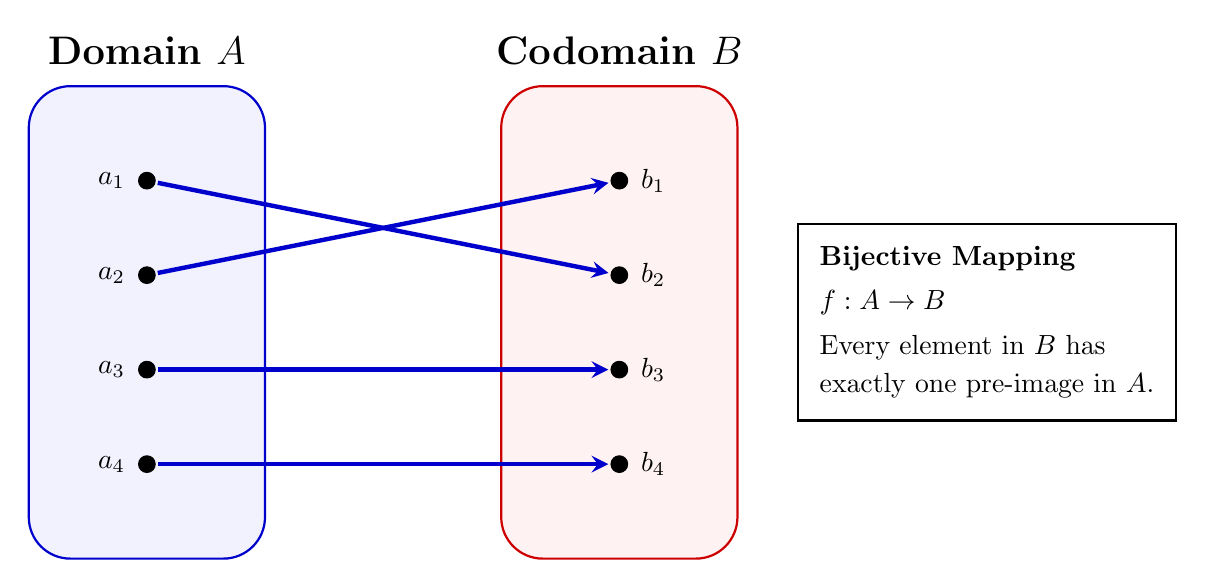
\begin{tikzpicture}[scale=1.5]
    % 1) Backgrounds
    \fill[blue!5, rounded corners=15pt] (-1, -2) rectangle (1, 2);
    \fill[red!5, rounded corners=15pt] (3, -2) rectangle (5, 2);
    
    % 2) Grid/Axes (Borders for the sets)
    \draw[thick, blue!80!black, rounded corners=15pt] (-1, -2) rectangle (1, 2);
    \draw[thick, red!80!black, rounded corners=15pt] (3, -2) rectangle (5, 2);
    
    % 3) Primary Plots (The mapping arrows)
    \draw[->, >=stealth, ultra thick, blue!80!black, shorten >=4pt, shorten <=4pt] (0, 1.2) -- (4, 0.4);
    \draw[->, >=stealth, ultra thick, blue!80!black, shorten >=4pt, shorten <=4pt] (0, 0.4) -- (4, 1.2);
    \draw[->, >=stealth, ultra thick, blue!80!black, shorten >=4pt, shorten <=4pt] (0, -0.4) -- (4, -0.4);
    \draw[->, >=stealth, ultra thick, blue!80!black, shorten >=4pt, shorten <=4pt] (0, -1.2) -- (4, -1.2);
    
    % 4) Nodes and Labels
    \node[black, font=\Large\bfseries] at (0, 2.3) {Domain $A$};
    \node[black, font=\Large\bfseries] at (4, 2.3) {Codomain $B$};
    
    % Domain Elements
    \filldraw[black] (0, 1.2) circle (2pt);
    \draw[thick] (0, 1.2) -- (-0.05, 1.2) node[left=2pt, black] {$\displaystyle a_1$};
    
    \filldraw[black] (0, 0.4) circle (2pt);
    \draw[thick] (0, 0.4) -- (-0.05, 0.4) node[left=2pt, black] {$\displaystyle a_2$};
    
    \filldraw[black] (0, -0.4) circle (2pt);
    \draw[thick] (0, -0.4) -- (-0.05, -0.4) node[left=2pt, black] {$\displaystyle a_3$};
    
    \filldraw[black] (0, -1.2) circle (2pt);
    \draw[thick] (0, -1.2) -- (-0.05, -1.2) node[left=2pt, black] {$\displaystyle a_4$};
    
    % Codomain Elements
    \filldraw[black] (4, 1.2) circle (2pt);
    \draw[thick] (4, 1.2) -- (4.05, 1.2) node[right=2pt, black] {$\displaystyle b_1$};
    
    \filldraw[black] (4, 0.4) circle (2pt);
    \draw[thick] (4, 0.4) -- (4.05, 0.4) node[right=2pt, black] {$\displaystyle b_2$};
    
    \filldraw[black] (4, -0.4) circle (2pt);
    \draw[thick] (4, -0.4) -- (4.05, -0.4) node[right=2pt, black] {$\displaystyle b_3$};
    
    \filldraw[black] (4, -1.2) circle (2pt);
    \draw[thick] (4, -1.2) -- (4.05, -1.2) node[right=2pt, black] {$\displaystyle b_4$};
    
    % Legend using single node multiline rule
    \node[align=left, draw=black, thick, fill=white, inner sep=8pt, anchor=west] at (5.5, 0) {
        \textbf{Bijective Mapping} \\[4pt]
        $\displaystyle f: A \to B$ \\[4pt]
        Every element in $B$ has \\[2pt]
        exactly one pre-image in $A$.
    };
\end{tikzpicture}
\end{center}

\subsection{Heuristics and Pitfalls}
\begin{itemize}
    \item \textbf{Heuristic for Injectivity:} Always start your proof with "Assume $f(a) = f(b)$". If the function involves absolute values, even powers ($x^2$), or periodic functions ($\sin(x)$), it is likely \textit{not} injective. Look for a counterexample immediately.
    \item \textbf{Heuristic for Surjectivity:} Treat the problem like an algebra equation. Set $f(x) = y$ and solve for $x$. If you can isolate $x$ and prove that this $x$ is always a valid member of the domain, you have proven surjectivity.
    \item \textbf{Pitfall - Confusing Codomain and Range:} The codomain is the set of \textit{potential} outputs defined by the function signature $f: A \to B$. The range (or image) is the set of \textit{actual} outputs. A function is only surjective if the range equals the codomain.
    \item \textbf{Pitfall - Assuming a Relation is a Function:} As seen in Problem 10.28, before checking if a mapping is one-to-one, you must verify it is a function. If an input maps to multiple outputs, it fails the vertical line test and is merely a relation.
\end{itemize}

\newpage
\section{Conceptual Synthesis and The "Big Picture"}

\subsection{Thematic Connections}
The central theme of this topic is \textbf{structural preservation and cardinality}. By classifying functions as injective, surjective, or bijective, we are fundamentally asking how a transformation alters the "size" and "distinguishability" of data. Injectivity ensures no data is lost (no two distinct inputs collapse into one). Surjectivity ensures the target space is fully reachable. Bijectivity ensures a perfect, reversible translation between two spaces. This unifies previous topics in set theory by providing a rigorous mechanism to compare sets without simply counting their elements.

\subsection{Forward and Backward Links}
\begin{itemize}
    \item \textbf{Backward Links:} This topic builds directly on the Cartesian product and relations. A function is simply a highly constrained relation (a subset of $A \times B$).
    \item \textbf{Forward Links:} Understanding bijections is the absolute bedrock for Abstract Algebra (where bijections that preserve operations are called \textit{isomorphisms}), Topology (where continuous bijections with continuous inverses are \textit{homeomorphisms}), and Measure Theory (where bijections are used to define the cardinality of infinite sets, such as proving $\R$ is uncountably infinite).
\end{itemize}

\section{Abstract Real-World Modeling (AI, ML, \& Quant Finance)}

\subsection{Concrete Scenarios}
\begin{enumerate}
    \item \textbf{Generative AI and Normalizing Flows:} In modern Machine Learning, Normalizing Flows are used to model complex probability distributions. They rely on applying a sequence of \textit{bijective} transformations to a simple base distribution (like a Gaussian). Because the transformations are bijective, the model can perfectly invert the mapping to generate new data, and the exact likelihood can be computed using the change-of-variables formula.
    \item \textbf{Quantitative Finance and Copulas:} In risk management, modeling the joint distribution of multiple assets requires separating the marginal distributions from the dependency structure. Sklar's Theorem uses the fact that the Cumulative Distribution Function (CDF) of a continuous random variable is a \textit{bijection} from $\R$ to the interval $(0, 1)$ to map any asset's returns into a uniform space, where a Copula function can model their correlation.
\end{enumerate}

\subsection{Model Problem Setup: Inverse Transform Sampling}
In Quantitative Finance, Monte Carlo simulations are heavily used to price complex derivatives. To simulate asset paths, we must generate random variables from arbitrary distributions using only a standard uniform random number generator. This relies entirely on the bijective properties of functions.

\textbf{Mathematical Framework:}
Let $(\Omega, \F, \Prob)$ be a probability space. Let $U$ be a random variable uniformly distributed on $(0, 1)$. 
Let $F: \R \to (0, 1)$ be a strictly increasing, continuous Cumulative Distribution Function (CDF) for some target financial variable (e.g., asset returns). 

Because $F$ is strictly increasing, it is \textbf{injective}. Because it is a continuous CDF bounded by $0$ and $1$, it is \textbf{surjective} onto $(0, 1)$. Therefore, $F$ is a \textbf{bijection}, and its inverse function $F^{-1}: (0, 1) \to \R$ is well-defined.

We define a new random variable $X = F^{-1}(U)$. We must prove that $X$ exactly follows the distribution $F$.
\begin{proof}
We evaluate the CDF of our generated variable $X$, denoted as $\Prob(X \le x)$:
\begin{align*}
\Prob(X \le x) &= \Prob(F^{-1}(U) \le x)
\end{align*}
Because $F$ is a strictly increasing bijection, applying $F$ to both sides of the inequality preserves the inequality direction:
\begin{align*}
\Prob(F^{-1}(U) \le x) &= \Prob(F(F^{-1}(U)) \le F(x)) \\
&= \Prob(U \le F(x))
\end{align*}
By the definition of the Uniform distribution on $(0, 1)$, for any value $k \in (0, 1)$, $\Prob(U \le k) = k$. Since $F(x) \in (0, 1)$, we have:
\begin{align*}
\Prob(U \le F(x)) &= F(x)
\end{align*}
Thus, $\Prob(X \le x) = F(x)$. The generated variable $X$ perfectly models the target financial distribution, entirely made possible by the bijective nature of $F$. $\blacksquare$
\end{proof}

\newpage
\section{Common Variations and Untested Concepts}

A standard concept in advanced mathematics not covered in the provided homework is the relationship between function composition and injectivity/surjectivity. 

\begin{theorem}
Let $f: A \to B$ and $g: B \to C$ be functions. If the composition $g \circ f: A \to C$ is injective, then the inner function $f$ must be injective.
\end{theorem}
\begin{proof}
We proceed by direct proof. Assume that $g \circ f$ is injective. We wish to show that $f$ is injective. 
Let $a_1, a_2 \in A$ and assume $f(a_1) = f(a_2)$. 
Since $f(a_1)$ and $f(a_2)$ are elements of $B$, we can apply the function $g$ to both sides of the equation:
\[ g(f(a_1)) = g(f(a_2)) \]
By the definition of function composition, this is equivalent to:
\[ (g \circ f)(a_1) = (g \circ f)(a_2) \]
Because we assumed that $g \circ f$ is injective, the equality of the outputs implies the equality of the inputs. Therefore:
\[ a_1 = a_2 \]
Since $f(a_1) = f(a_2) \implies a_1 = a_2$, the function $f$ is injective. $\blacksquare$
\end{proof}
\textit{Note:} The outer function $g$ does \textit{not} need to be injective. This is a common trap for students.

\section{Advanced Diagnostic Testing: "Find the Flaw"}

Below are five proofs that appear rigorous but contain a subtle, fatal logical flaw. Your task as the grader is to identify the error.

\subsection{Flawed Proof 1}
\textbf{Problem:} Prove that the function $f: \R \to \R$ defined by $f(x) = e^x$ is surjective. \\
\textbf{Flawed Proof:} Let $y \in \R$. We must find an $x \in \R$ such that $f(x) = y$. We set $e^x = y$. Taking the natural logarithm of both sides, we obtain $x = \ln(y)$. Since the natural logarithm is a well-defined mathematical function, $x$ exists and is a real number. Thus, for every $y$, there is an $x$ such that $f(x) = y$. Therefore, $f$ is surjective. $\blacksquare$

\subsection{Flawed Proof 2}
\textbf{Problem:} Let $f: A \to B$ and $g: B \to C$ be functions. Prove that if the composition $g \circ f$ is injective, then $g$ is injective. \\
\textbf{Flawed Proof:} Assume $g \circ f$ is injective. We want to show $g$ is injective. Let $b_1, b_2 \in B$ such that $g(b_1) = g(b_2)$. Since $b_1, b_2 \in B$, there exist $a_1, a_2 \in A$ such that $f(a_1) = b_1$ and $f(a_2) = b_2$. Substituting these into our equation gives $g(f(a_1)) = g(f(a_2))$, which means $(g \circ f)(a_1) = (g \circ f)(a_2)$. Because $g \circ f$ is injective, this implies $a_1 = a_2$. Applying $f$ to both sides yields $f(a_1) = f(a_2)$, so $b_1 = b_2$. Thus, $g$ is injective. $\blacksquare$

\subsection{Flawed Proof 3}
\textbf{Problem:} Let $f: A \to B$ be a function, and let $X, Y \subseteq A$. Prove that $f(X \setminus Y) \subseteq f(X) \setminus f(Y)$. \\
\textbf{Flawed Proof:} Let $z \in f(X \setminus Y)$. By definition, there exists an element $x \in X \setminus Y$ such that $f(x) = z$. Since $x \in X \setminus Y$, we know that $x \in X$ and $x \notin Y$. Because $x \in X$, it follows that $f(x) \in f(X)$. Because $x \notin Y$, it follows that $f(x) \notin f(Y)$. Therefore, $z = f(x) \in f(X) \setminus f(Y)$. This proves the subset inclusion. $\blacksquare$

\subsection{Flawed Proof 4}
\textbf{Problem:} Prove that the function $f: \Z \to \Z$ defined by $f(n) = 3n$ is a bijection. \\
\textbf{Flawed Proof:} First, we show injectivity. Let $f(a) = f(b)$. Then $3a = 3b$, which implies $a = b$. Thus, $f$ is injective. Next, we show surjectivity. Let $y \in \Z$. We need to find an $x \in \Z$ such that $f(x) = y$. We set $3x = y$ and solve for $x$ to get $x = y/3$. Since $y$ is an integer, we have found our $x$. Because we can find an $x$ for every $y$, $f$ is surjective. Since $f$ is both injective and surjective, it is a bijection. $\blacksquare$

\subsection{Flawed Proof 5}
\textbf{Problem:} Let $A = \{1, 2, 3\}$ and $B = \{4, 5\}$. Prove that there exists a surjective function $f: A \to B$ that is also injective. \\
\textbf{Flawed Proof:} We construct the function explicitly. Let $f(1) = 4$ and $f(2) = 5$. To ensure injectivity, we must map distinct elements of $A$ to distinct elements of $B$. Since $1 \neq 2$ and $f(1) \neq f(2)$, the function is injective. Furthermore, the image of $f$ is $\{4, 5\}$, which is exactly the codomain $B$. Thus, $f$ is surjective. Since $f$ is both injective and surjective, we have proven its existence. $\blacksquare$

\vspace{1cm}
\subsection{Solution Key: The Flaws Revealed}
\begin{itemize}
    \item \textbf{Flaw 1:} The proof assumes $\ln(y)$ is defined for all $y \in \R$. The natural logarithm is only defined for $y > 0$. If $y = -1 \in \R$, there is no real $x$ such that $e^x = -1$. Thus, $f$ is not surjective.
    \item \textbf{Flaw 2:} The proof falsely assumes that for any $b_1, b_2 \in B$, there exist $a_1, a_2 \in A$ such that $f(a_1) = b_1$ and $f(a_2) = b_2$. This assumes $f$ is surjective, which is not given. The theorem itself is false.
    \item \textbf{Flaw 3:} The deduction "$x \notin Y \implies f(x) \notin f(Y)$" is invalid unless $f$ is injective. If $f$ is not injective, there could be another element $y \in Y$ such that $f(x) = f(y)$, meaning $f(x) \in f(Y)$ even though $x \notin Y$.
    \item \textbf{Flaw 4:} The proof claims $x = y/3$ is an integer just because $y$ is an integer. If $y = 1 \in \Z$, then $x = 1/3 \notin \Z$. Thus, $f$ is not surjective.
    \item \textbf{Flaw 5:} The constructed $f$ is not a valid function from $A$ to $B$ because it fails to assign an output to the element $3 \in A$. If we attempt to define $f(3)$, it must map to either $4$ or $5$, which immediately violates injectivity. By the Pigeonhole Principle, no such function can exist.
\end{itemize}

\end{document}